%---------------------------------------------------
% کلاس سند: article برای اسناد متنی، با اندازه کاغذ A4 و فونت پایه 16
\documentclass[a4paper,16pt]{article}

% بسته‌های ریاضی برای معادلات و نمادهای پیشرفته
\usepackage{amsmath, amssymb, amstext}

% بسته رنگ برای استفاده از رنگ در متن یا محیط‌ها
\usepackage{xcolor,tcolorbox}


% بسته گرافیک برای درج تصاویر
\usepackage{graphicx}

% تنظیمات حاشیه صفحه
\usepackage{geometry}

% بسته لینک‌دهی (هایپرلینک‌ها)
\usepackage{hyperref}

% بسته صفحه‌آرایی برای تنظیم هدر و فوتر
\usepackage{fancyhdr}


% بسته xepersian برای پشتیبانی از زبان فارسی با XeLaTeX


% تعیین فونت فارسی (فایل فونت باید موجود باشد یا در سیستم نصب باشد)
\usepackage{xepersian}
\settextfont{B Nazanin}

\setlatintextfont{Times New Roman}

% تنظیم اندازه حاشیه‌ها از هر طرف برابر با 1 اینچ
\geometry{margin=1in}

% تنظیم سبک fancy برای سربرگ و پاورقی
\pagestyle{fancy}

% سمت چپ هدر: مشخص‌کننده سری تمرین و نام درس
\lhead{تمرین سری ششم درس مکانیک تحلیل }

% وسط هدر: نام دانشکده
\chead{دانشکده فیزیک دانشگاه صنعتی خواجه نصیرالدین طوسی}

% سمت راست هدر: تاریخ روز به‌صورت خودکار
\rhead{\today}

% پایین صفحه: شماره صفحه
\cfoot{\thepage}

% شروع سند
\begin{document}
	

	
	% صفحه عنوان (بدون هدر و فوتر)
	\thispagestyle{empty}
	\begin{center}
		% لوگوی دانشگاه (باید فایل تصویر در مسیر پروژه باشد)
		
\includegraphics[width=0.5\textwidth]{../../../images/image-E_5/image-1.png} \\[10pt] 
		
		% عنوان سند
		\textbf{\LARGE عنوان:تمرین سری ششم}\\[20pt]
		
		% نیم‌سال تحصیلی
		\textbf{\LARGE نیم‌سال تحصیلی:4041 }\\[10pt]
		
		% نام مدرس درس
		\textbf{\Large مدرس: دکتر محمد انصاری‌فرد}\\[10pt]
		
		% مبحث تمرین 
		\textbf{\Large مبحث تمرین:لاگرانژي   }\\[10pt]
		
		% مهلت تحویل تمرین
		\textbf{\Large مهلت تحویل:۱۹دی }
	\end{center}
	
	% صفحه جدید برای ادامه سند
	\newpage
	
	% ایجاد فهرست مطالب به‌صورت خودکار (براساس \section و \subsection و ...)
	\tableofcontents
	\newpage
	
	\begin{tcolorbox}[
		colback=yellow!15,
		colframe=orange!80!black,
		title=\textbf{تذکر مهم},
		fonttitle=\bfseries,
		boxrule=0.8pt,
		arc=4mm,
		left=6pt,
		right=6pt,
		top=6pt,
		bottom=6pt
		]
		حل \textbf{تمامی سوالات این تمرین صرفاً باید با استفاده از فرمالیسم لاگرانژ و معادلات اویلرلاگرانژ} انجام شود و استفاده از روش‌های نیوتنی مجاز نیست.
	\end{tcolorbox}
	
	\section{سوال اول}
		معادلات حرکت پرتابه را در میدان گرانشی یکنواخت و بدون مقاومت هوا بدست آورید
	\section{سوال دوم}
	
	ذره ای در امتداد یک جوی چرخزاد صاف آزادانه حرکت میکند.سطح این چرخزاد در قالب این معادلات پارامتری بیان میشود
\\
\[
x=\frac{a}{4}\bigl(2\theta+\sin\theta\bigr)
\]
\[
y=\frac{a}{4}\bigl(1-\cos(2\theta)\bigr)
\]که در آن $\theta \in [0,\pi]$ و $a$ ثابت است.
لانگرانژی و معادلات حرکت ذره را بیابید.

	
	\section{سوال سوم}
	
	معادلات ماشین آتوود زیر را بدست آورید.
		\begin{figure}[h]
		\centering
		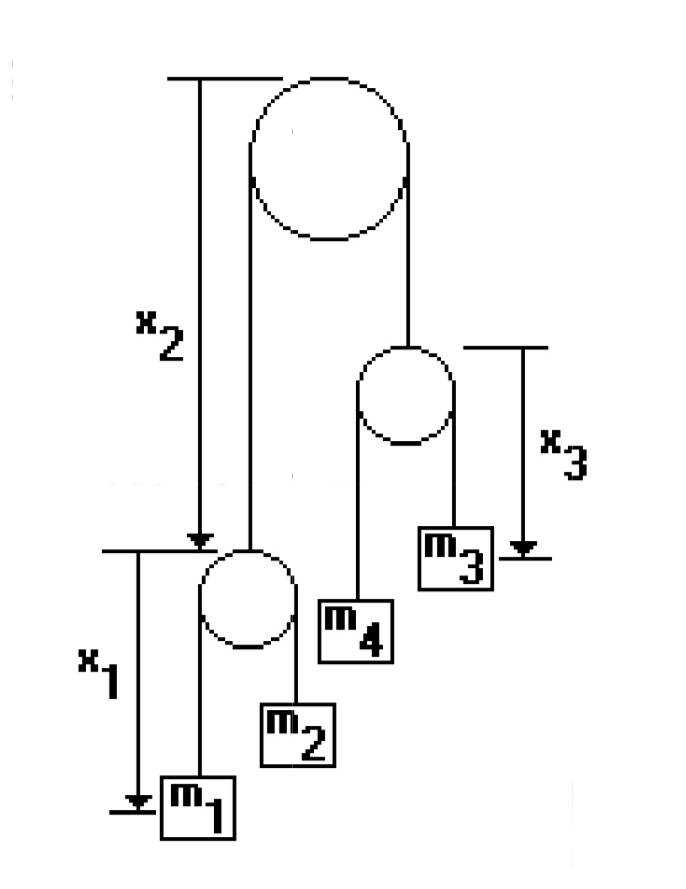
\includegraphics[width=0.5\textwidth]{../../../images/image-E_6/image-2.png}
	\end{figure}
	
	\section{سوال چهارم}
	
	
	یک ذره به جرم \(m\) در فضای سه‌بعدی قرار دارد و تحت تأثیر پتانسیل
	\[
	V(x, y, z) = \frac{1}{2} k (x^2 + y^2 + z^2)
	\]
	قرار دارد.
	
	\begin{enumerate}
		\item تابع لاگرانژی \(L = T - V\) را برای ذره بنویسید، که در آن انرژی جنبشی \(T\) برابر است با
		\[
		T = \frac{1}{2} m (\dot{x}^2 + \dot{y}^2 + \dot{z}^2).
		\]
		
		\item معادلات اویلرلاگرانژ برای مختصات \(x, y, z\) بدست آورید:
		\[
		\frac{d}{dt} \left( \frac{\partial L}{\partial \dot{q}_i} \right) - \frac{\partial L}{\partial q_i} = 0, \quad q_i = x, y, z.
		\]
		
		\item معادلات حرکت را برای شرایط اولیه دلخواه حل کنید؛ مثلاً ذره از مبدأ با سرعت اولیه \(v_0\) در جهت \(x\) حرکت می‌کند.
	\end{enumerate}
	\section{سوال پنجم}
	یک
	یک ذره به جرم \(m\) روی یک صفحه افقی بدون اصطکاک حرکت می‌کند و با یک فنر شعاعی به مبدأ متصل است. انرژی پتانسیل فنر به صورت زیر است:
	\[
	V(r) = \frac{1}{2} k r^2
	\]
	
	\begin{enumerate}
		\item تابع لاگرانژی \(L = T - V\) را در مختصات قطبی \((r, \theta)\) بنویسید، که انرژی جنبشی برابر است با
		\[
		T = \frac{1}{2} m (\dot{r}^2 + r^2 \dot{\theta}^2).
		\]
		
		\item معادلات اویلرلاگرانژ برای \(r\) و \(\theta\) بدست آورید:
		\[
		\frac{d}{dt} \left( \frac{\partial L}{\partial \dot{q}_i} \right) - \frac{\partial L}{\partial q_i} = 0, \quad q_i = r, \theta.
		\]
		
		\item ثابت حرکت زاویه‌ای (گشتاور زاویه‌ای) را تعیین کنید و معادله حرکت شعاعی را به شکل ساده بیان کنید.
	\end{enumerate}
	\section{سوال ششم}
	
	یک ذره به جرم \(m\) روی یک سطح شیبدار بدون اصطکاک حرکت می‌کند. زاویه شیب سطح نسبت به افق \(\alpha\) است و نیروی گرانش \(mg\) عمل می‌کند.
	
	\begin{enumerate}
		\item تابع لاگرانژی \(L = T - V\) را برای مختصات \(x\) (در امتداد سطح) بنویسید. انرژی جنبشی و پتانسیل به ترتیب:
		\[
		T = \frac{1}{2} m \dot{x}^2, \quad V = mg x \sin\alpha.
		\]
		
		\item معادله اویلرلاگرانژ برای \(x(t)\) را بدست آورید:
		\[
		\frac{d}{dt} \left( \frac{\partial L}{\partial \dot{x}} \right) - \frac{\partial L}{\partial x} = 0
		\]
		
		\item معادله حرکت ذره را حل کنید و سرعت آن را به عنوان تابع زمان پیدا کنید، اگر ذره در ابتدا ساکن بوده باشد.
	\end{enumerate}
	\section{سوال امتیازی}
	
	یک ذره به جرم \(m\) در میدان گرانشی یک جرم مرکزی \(M\) قرار دارد. میدان گرانشی توسط متریک شوارتزشیلد داده شده است:
	\[
	ds^2 = -\left(1-\frac{2GM}{c^2 r}\right)c^2 dt^2 + \left(1-\frac{2GM}{c^2 r}\right)^{-1} dr^2 + r^2 (d\theta^2 + \sin^2\theta\, d\phi^2)
	\]
	
	فرض کنید حرکت ذره در صفحه \(\theta = \pi/2\) صورت می‌گیرد.
	\\
	
	\noindent
	متریک $g_{\mu\nu}$ مشخص‌کننده ساختار هندسی فضازمان بوده و فاصله فضازمانی $ds^2$ را تعیین می‌کند.
	زمان ویژه $\tau$ زمانی است که توسط ناظر هم‌حرکت با ذره اندازه‌گیری می‌شود و از رابطه
	\[
	d\tau^2 = -\frac{1}{c^2} ds^2
	\]
	به‌دست می‌آید.
	\vspace{10pt}
	
	
	\begin{enumerate}
		\item لاگرانژی ذره را بنویسید:
		\[
		L = \frac{1}{2} g_{\mu\nu} \dot{x}^\mu \dot{x}^\nu,
		\]
		که \(\dot{x}^\mu = \frac{dx^\mu}{d\tau}\) است و \(\tau\) زمان محلی ذره است.
		
		\item معادلات اویلرلاگرانژ را برای مختصات \(r\) و \(\phi\) بدست آورید:
		\[
		\frac{d}{d\tau} \left( \frac{\partial L}{\partial \dot{r}} \right) - \frac{\partial L}{\partial r} = 0, \quad
		\frac{d}{d\tau} \left( \frac{\partial L}{\partial \dot{\phi}} \right) - \frac{\partial L}{\partial \phi} = 0
		\]
		
		\item ثابت‌های حرکت زاویه‌ای و انرژی را تعیین کنید:
		\[
		\ell = r^2 \dot{\phi}, \quad E = \left(1-\frac{2GM}{c^2 r}\right) \dot{t} c^2
		\]
		
		\item معادله شعاعی حرکت را به صورت:
		\[
		\left(\frac{dr}{d\tau}\right)^2 = E^2/c^2 - \left(1-\frac{2GM}{c^2 r}\right)\left(c^2 + \frac{\ell^2}{r^2}\right)
		\]
		بدست آورید.
		
		\item با فرض \(r \gg 2GM/c^2\) و سرعت ذره \(v \ll c\)، تقریب نیوتنی بزنید و معادله حرکت را به شکل کلاسیک:
		\[
		m \frac{d^2 \mathbf{r}}{dt^2} = - \frac{GM m}{r^2} \hat{\mathbf{r}}
		\]
		کاهش دهید.
	\end{enumerate}
	\vspace{10pt}
	\textbf{موفق باشید.}
\end{document}
